\documentclass[12pt]{article}    
    
 	\usepackage{amsfonts}
 	\usepackage{graphicx}

	\title{Práctica 3 TALF}
    \author{Jesús Alcázar Pérez 2ºA Ingeniería Informática}
    \date{\today}

	\addtolength{\topmargin}{-4cm}
    \addtolength{\textheight}{4cm}
    %\usepackage[spanish]{babel}
    \usepackage[a4paper, margin=3cm, top=5mm, bottom=15mm]{geometry}
    \usepackage{graphicx}
    \usepackage{tikz}
	
\begin{document}


\maketitle
\thispagestyle{plain}

\section{Turing Machine example done with JFLAP}
\begin{figure}[htp]
\centering
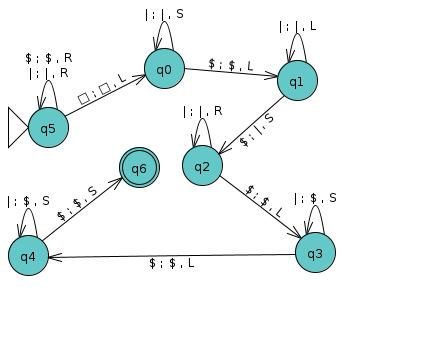
\includegraphics[scale=0.50]{Entrega/Ejercicio3.4_MT.jpg}
\caption{TM that sums 2 values}
\end{figure}


\section{Requested Recursive function and an Octave capture}
\centering
addition\_3 = $<<\pi^1_1|\sigma(\pi^3_3)>| \sigma(\pi^4_4)>$ 
\begin{figure}[htp]
\centering
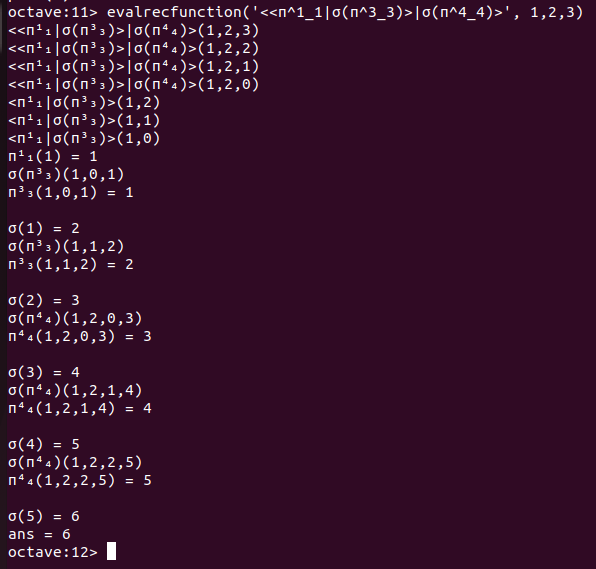
\includegraphics[scale=0.40]{Entrega/CapturaAddition3Rec.png}
\caption{Addition3 in Octave execution}
\label{}
\end{figure}


\newpage
\section{WHILE program that computes the sum of 3 values}
\centering
\begin{verbatim}
 Q: (3, 4, s)
 s:
   while X1 != 0 do
     X2 := X2 + 1;
     X1 := X1 - 1
   od;
   X4 := X2;
   while X2 != 0 do
     X3 := X3 + 1;
     X2 := X2 - 1
   od;
   X1 := X4
   
   //Done with verbatim due to error in package whilecode

\end{verbatim}

\end{document}